\documentclass[runningheads]{llncs}

\usepackage[T1]{fontenc}
\usepackage{newtxtext}
\usepackage[varvw]{newtxmath}
\usepackage{graphicx}
\usepackage{booktabs}
\usepackage{url}
\usepackage{array}
\usepackage{amsmath}
\usepackage{xcolor}
\renewcommand\UrlFont{\color{black}\rmfamily}

\begin{document}

% =========================================================
% TITLE
% =========================================================

\title{Exploring Physiological Stress Patterns During Urban Public
Transport Commutes Using Wearable Sensors and Unsupervised Learning:
A Pilot Study}

\titlerunning{Physiological Stress Patterns in Urban Public Transport}
\author{Melany Cahuana-Nina\inst{1} \and Andrea L. Cuela\inst{1} \and Rushell Vanessa Zavalaga Orozco\inst{1}}
\authorrunning{M. Cahuana-Nina et al.}
\institute{Universidad Nacional de San Agust\'{i}n de Arequipa, Arequipa, Peru\\
\email{\{mcahuanan,acuela,rzavalaga\}@unsa.edu.pe}}


\maketitle

\begin{abstract}
Wrist-worn wearables are increasingly proposed to study commuters' stress, yet in-the-wild studies rarely separate physiology from context and motion artefacts. We present a reproducible pipeline that converts the raw 20-byte Bluetooth packets of a research-grade wristband, logged with smartphone GPS and microphone level, into synchronised 30-s windows, and evaluate it on 15 sessions (6.2~h of windows with 50\,\% overlap) recorded by four volunteers on public buses. As the packet format is undocumented, we infer and validate four decoded streams (temperature, acceleration, photoplethysmography and one of two electrodermal packet formats), with effective sampling rates within 0.02\,\% of nominal and no packet loss. With analyses specified beforehand, leave-one-participant-out and leave-one-session-out validation, block-permutation tests and Holm correction, we find that (i)~the wrist accelerometer alone detects whether the bus is stopped or moving (AUC 0.83, 95\,\% CI 0.77--0.89; Holm-adjusted $p=0.004$); (ii)~physiology alone (heart rate, HRV, skin temperature, electrodermal activity) predicts traffic, noise and exposure proxies in unseen persons no better than chance (balanced accuracy 0.21--0.38 vs.\ 0.33 expected; all $p\geq0.25$), whereas adding vibration features raises it to 0.44 (traffic) and 0.41 (noise); (iii)~a heart-rate response to noise bursts cannot be established (+1.7~bpm, 95\,\% CI $-0.7$ to $+3.6$; Bayes factor $\approx1$, i.e.\ inconclusive); and (iv)~vehicle motion inflates HRV and tends to reduce valid pulse estimates. We discuss threats to validity and give actionable recommendations for stress-sensing studies in transit.
\keywords{wearable sensing \and public transport \and Internet of Things \and data quality \and accelerometer \and negative results}
\end{abstract}

\section{Introduction}
Public-transport riders are exposed daily to congestion, noise and crowding, and wearables make it possible to record physiology during real trips. A tempting inference is that physiological changes on a bus reflect the ride context. However, a wrist sensor on a moving vehicle also measures the vehicle: vibration corrupts photoplethysmography (PPG), skin sensors need minutes to settle, devices differ between people, and every session has its own baseline. Studies that cluster physiological windows and compare the clusters with context labels can therefore report associations that are really differences between sessions or people. Our contributions are:
\begin{enumerate}
\item A reproducible pipeline from raw Bluetooth Low Energy (BLE) packets of a research-grade wristband to synchronised 30-s windows. As the packet format is undocumented, we infer the layout of four streams and validate it with physical criteria (Sect.~\ref{sec:decoding}).
\item A detector of \emph{vehicle state} (stopped vs.\ moving) that uses only the wrist accelerometer, validated against smartphone GPS speed on held-out persons and sessions (AUC 0.83--0.85).
\item Pre-specified negative results: physiology alone does not predict traffic, noise or exposure proxies above chance in unseen persons, no heart-rate response to noise bursts can be established, and an apparent cluster--context association is largely a between-session effect.
\item Data-quality findings and a table of actionable recommendations (Table~\ref{tab:recs}).
\end{enumerate}

\section{Related Work}
WESAD~\cite{schmidt2018} is a reference dataset for wearable stress and affect detection with the Empatica E4 (BVP, EDA, temperature, acceleration), but its protocol was run in the laboratory. Iqbal et al.~\cite{iqbal2022} compared unsupervised algorithms for physiological stress detection. A systematic review concluded that the generalisation of stress models to new people remains an open problem~\cite{vos2023}, and device-specific limitations hamper the transfer of models between wearables~\cite{amin2025}. In transit, Bosch et al.~\cite{bosch2025} released a georeferenced dataset combining experience sampling, GPS and cardiac activity during real public-transport trips, and Wang et al.~\cite{wang2023} related personal noise exposure during commutes to self-reported stress. Validation studies of the E4 against ECG show that mean inter-beat interval is reliable but RMSSD is difficult to obtain under motion~\cite{schuurmans2020}, and that in a driving setting frequency-domain HRV needs caution and the electrodermal signal was unreliable~\cite{costantini2023}; a recent preprint stresses the difficulty of separating psychological stress from physical exertion in wearable signals~\cite{bosch2026}. We differ in three respects: we start from undocumented raw packets, we fix the evaluation protocol in advance and control multiplicity, and we report null results with their uncertainty.

\section{Data and Pipeline}
\begin{figure}[t]
\centering
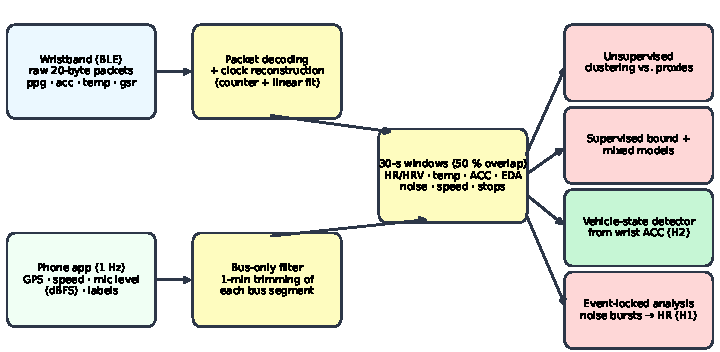
\includegraphics[width=0.92\textwidth]{figs/fig1_pipeline.pdf}
\caption{Pipeline. Wristband packets and smartphone measurements are decoded, synchronised through timestamps, restricted to bus segments and summarised in 30-s windows, which feed four analyses (H1, H2: pre-specified hypotheses).}
\label{fig:pipeline}
\end{figure}

\subsection{Data collection}
Four adult volunteers (P1--P4) recorded bus and minibus trips in Arequipa, Peru, between 18 and 30 September 2026 (04:00--20:00), using an Empatica E4 wristband streaming over BLE to a smartphone application. The application logged, once per second, GPS position, accuracy and speed and the microphone root-mean-square level in dBFS (no audio is stored), together with a transport-mode label and optional event marks. Three wristbands were used for four people (P1 and P4 shared one). Participants gave informed consent; identifiers are pseudonymous.

\subsection{Session selection and bus filtering}
\label{sec:selection}
Of 17 recorded sessions, two were excluded for technical reasons fixed before analysis: the wristband stream lasted 20~s of a 16-min session in one, and the stream file was empty in the other. The automatic transport-mode label was unreliable and heterogeneous (one participant was always on a bus but the label stayed ``walking''; others switched to ``walking'' to mark the end of a recording), so we kept only bus time: all samples of P1 and four full sessions of P2 (confirmed by the participant), and only samples labelled \emph{bus} elsewhere; the first and last 60~s of every bus segment were discarded (boarding and alighting). Rest, waiting and walking were not used because their labels were inconsistent across participants. This selection can bias results (Sect.~\ref{sec:threats}), so we repeat the key detector analysis using only windows whose \emph{bus} label was used as recorded (Sect.~\ref{sec:h2}). Two legacy sessions of P2 lack a usable microphone signal and trip metadata and are used only where noise is not required. The dataset has 1\,498 windows (Table~\ref{tab:data}).

\begin{table}[t]
\caption{Dataset after bus filtering. Windows last 30~s with a 15-s step (50\,\% overlap); hours are computed from the step. ``EDA'' and ``Noise'' are the numbers of windows with float-format electrodermal data and with a valid microphone level.}
\label{tab:data}
\centering
\setlength{\tabcolsep}{7pt}
\begin{tabular}{lrrrrr}
\toprule
Participant & Sessions & Windows & Hours & EDA & Noise\\
\midrule
P1 & 3 & 313 & 1.3 & 313 & 307\\
P2 & 7 & 847 & 3.5 & 0 & 240\\
P3 & 4 & 265 & 1.1 & 265 & 265\\
P4 & 1 & 73 & 0.3 & 73 & 73\\
\midrule
Total & 15 & 1\,498 & 6.2 & 651 & 885\\
\bottomrule
\end{tabular}
\end{table}

\subsection{Decoding undocumented packets}
\label{sec:decoding}
Each logged record contains a channel name, a wall-clock timestamp and a 20-byte payload. The wristband transmits four sensor channels (temperature, acceleration, PPG and electrodermal activity, EDA); the EDA channel arrives in \emph{two} packet formats, so Table~\ref{tab:decoding} lists five layouts. We inferred each layout and checked it against physical expectations. Every packet carries a counter that never takes the value 0 (range 1--63 for PPG, 1--255 otherwise); packet loss is detected from counter gaps, using arrival time to resolve wrap-arounds. Sample times are reconstructed by a robust linear fit between sample index and arrival time, which removes BLE jitter.

\begin{table}[t]
\caption{Inferred packet layouts and validation. Rates are effective sampling rates from the fit; none of the channels shows packet loss. The EDA channel has two formats; \emph{only the float format is decoded and used}.}
\label{tab:decoding}
\centering
\footnotesize
\setlength{\tabcolsep}{3pt}
\begin{tabular}{>{\raggedright\arraybackslash}p{1.95cm}>{\raggedright\arraybackslash}p{4.6cm}>{\raggedright\arraybackslash}p{1.75cm}>{\raggedright\arraybackslash}p{3.0cm}}
\toprule
Channel & Layout (20 bytes) & Effective rate & Validation\\
\midrule
Temperature & $8\times$ uint16 little-endian; $T[^\circ\mathrm{C}] = 0.02\cdot\mathrm{raw} - 273.15$ & 4.000 Hz & 31--35~$^\circ$C, smooth\\
Accelerometer & $6\times(x,y,z)$ int8; $a[\mathrm{g}] = v/64$ & 32.003 Hz & $|a|\approx1$~g at rest\\
PPG & 11 samples, 14 bit signed, MSB first, in the first 154 bits; 6-bit counter & 64.006 Hz & Dominant 1.15--1.75 Hz spectral peak\\
EDA, float format & $4\times$ float32 little-endian ($\mu$S); one packet per 2~s & 0.500 Hz & 0.4--7.5 $\mu$S, plausible\\
EDA, ``type A'' & $6\times24$ bit = 10-bit signal (stored in a 12-bit field) + 12-bit baseline code that changes in steps of 9; one packet per 1.5~s (4 Hz) & 4 Hz & Not converted to $\mu$S; \emph{excluded}\\
\bottomrule
\end{tabular}
\end{table}

The type-A format carries a 10-bit signal and an automatic-baseline code that changes in exact steps of 9 units, whose jump in signal units is consistent across devices, and its variability correlates with motion, but a conversion to $\mu$S could not be found (a model $\mathrm{EDA}=k/(\mathrm{signal}+c\cdot\mathrm{code}+d)$ failed across sessions). \textbf{It is excluded from all analyses.} One participant's wristband emitted only this format, so electrodermal analyses use three participants.

\subsection{Windows, features and signal processing}
For each 30-s window (15-s step) we compute: heart rate (HR) from PPG band-passed with a zero-phase 3rd-order Butterworth filter (0.5--8~Hz; 0.5--4~Hz for beats), using beat detection and the dominant spectral peak (0.7--3~Hz); RMSSD and SDNN from inter-beat intervals within 0.4--1.5~s and $\pm30\,\%$ of the median; skin temperature mean and slope; accelerometer-magnitude statistics and band powers (Welch, 0.3--16~Hz); and mean EDA and slope. Windows need at least 80\,\% of the expected PPG and accelerometer samples; HR is valid when at least 15 beats are found and both HR estimates agree within 10~bpm (85\,\% of windows). From the phone we compute the equivalent noise level (Leq, dBFS; $-120$ dBFS treated as missing), the fraction of time with GPS speed below 1~km/h, and mean speed. Features are log-transformed where skewed and standardised within participant. Full settings are in the Supplement (S1).

\emph{Overlapping windows.} Because consecutive windows share 50\,\% of their samples, rows are not independent. We therefore (a) never split windows of one session between training and test sets (validation holds out whole participants or sessions), (b) permute labels by circular shifts within each session and bus segment, which preserves their autocorrelation, and (c) fit mixed models on non-overlapping windows only. These choices are conservative: the block-permutation null of our best detector has a mean AUC of 0.57 rather than 0.50.

\subsection{Context proxies}
Because no direct ground truth of stress exists, we define context \emph{proxies} that do not depend on physiology: a \emph{traffic proxy} (fluid: $<$10\,\% of the window stopped; congested: $\geq$50\,\%; moderate otherwise; 504/319/439 windows), a \emph{noise proxy} (low/medium/high terciles of Leq \emph{within each participant}, since every phone microphone has its own gain) and an \emph{exposure proxy} combining both. They label the ride context, not stress. The traffic proxy is physically coupled to vibration (Spearman $-0.54$ between fraction stopped and the log SD of acceleration over all windows; $-0.47$ to $-0.77$ within participants).

\section{Evaluation Protocol}
Analyses were specified before they were run (protocol files accompany the code) and thresholds were not changed after seeing results. We distinguish: unsupervised clustering (K-Means, Gaussian mixtures, Ward, DBSCAN; $k=2$--6; standardisation within participant); a supervised upper bound (random forest, 100 trees, minimum leaf size 5, balanced class weights; and logistic regression) predicting the proxies from physiological features; linear mixed models with a random intercept per session; and two confirmatory hypotheses, H1 (cardiac response to noise bursts) and H2 (vehicle-state detection from the wrist accelerometer). Two further analyses (pulse validity vs.\ vehicle state; speed regression) are exploratory. Generalisation is estimated by leave-one-participant-out (LOPO) and leave-one-session-out (LOSO) validation~\cite{gholami2020}; 95\,\% CIs come from bootstrapping whole sessions; significance from block-permutation tests~\cite{ojala2010} (200--2000 permutations). \emph{Multiplicity.} Family~1 (confirmatory) contains H1, H2 and the six physiology-only classifier cells (8 tests), controlled with the Holm procedure~\cite{holm1979}; the three cells that include vibration features form an exploratory Family~2 (Holm over 3 tests); all other analyses are descriptive and uncorrected. Random seeds are fixed (0). Software: Python 3.13.9, NumPy 2.3.5, pandas 2.3.3, SciPy~\cite{virtanen2020} 1.16.3, scikit-learn~\cite{sklearn2011} 1.7.2, statsmodels~\cite{seabold2010} 0.14.5.

\section{Results}
\subsection{Decoded signals}
Decoded signals from one session are shown in the Supplement (Fig.~S1). Effective rates are within 0.02\,\% of nominal and counters reveal no lost packets, which strongly supports the inferred layouts for temperature, acceleration and PPG. HR from PPG is physiologically plausible (typically 60--105~bpm), but no external reference (e.g., ECG) was available, so its absolute accuracy remains unverified and constitutes a major limitation (Sect.~\ref{sec:threats}).

\subsection{Unsupervised structure mostly reflects sessions}
Using HR, HRV and skin temperature only (four participants, 1\,267 windows), K-Means with $k=6$ agrees with the traffic proxy at NMI $0.013$ (block-permutation $p=0.22$) and with the noise proxy at $0.023$ ($p=0.11$); silhouette is 0.17--0.24 and bootstrap stability ARI 0.4--0.6. When the accelerometer variability is included, NMI rises to 0.063 for traffic (null mean 0.018, $p<0.001$): the structure appears only when vibration is available. With global normalisation clusters separate people instead. Adding EDA (three participants, windows $\geq$300~s after sensor start) gives NMI 0.13 with the traffic proxy against a null mean of 0.11 ($p=0.037$, uncorrected), which looked like a gain; however these clusters align far more with the recording \emph{session} ($k=6$: NMI with session 0.36--0.43) than with traffic (0.12--0.14). Within sessions the cluster--traffic NMI falls to 0.06--0.10, and the traffic proxy itself is partly determined by the session (NMI 0.14 without EDA, 0.27 with). EDA also decays during sensor warm-up (from about 7 to 2~$\mu$S in one night session).

\subsection{Physiology alone does not predict context across persons}
Table~\ref{tab:classifier} gives the supervised upper bound. With HR, HRV and skin temperature (and EDA in analysis~B), a random forest evaluated on a left-out participant is at or below chance for all three proxies: balanced accuracy 0.30 (traffic), 0.34 (noise) and 0.24 (exposure) in analysis~A, and 0.34, 0.38 and 0.21 in analysis~B; all CIs for traffic and noise include 0.33 and all permutation $p$ values are $\geq0.25$ (Holm-adjusted $p=1$). The 95th percentile of the permutation null is 0.34--0.43 for traffic and noise (0.29--0.32 for exposure), so only accuracies above these values could have been detected. Predictive power appears only when vibration features are added: 0.44 for traffic ($p=0.001$, Holm over the exploratory family $p=0.003$) and 0.41 for noise ($p=0.003$, Holm $0.006$) in analysis~A, and 0.42 for traffic in analysis~B (Holm $0.012$). Exposure stays below chance in every configuration. Removing the movement-explained part of HR and RMSSD does not help. Leave-one-session-out validation gives the same picture (analysis~A, traffic: 0.35, 95\,\% CI 0.28--0.41, without vs.\ 0.46, 0.39--0.52, with vibration; noise: 0.33 vs.\ 0.41). Per-participant and per-session accuracies and confusion matrices are in the Supplement (S3--S4).

\begin{table}[t]
\caption{Random forest, leave-one-participant-out balanced accuracy (BA; chance $=0.33$) with 95\,\% bootstrap CI over sessions, and block-permutation $p$ (uncorrected; $^\dagger$: 1000 permutations, others 200). A: four participants, no EDA ($n=634$--$1054$ windows). B: three participants with EDA after 300~s of warm-up ($n=398$--$411$). ``Residual'' removes the part of HR and ln RMSSD explained by accelerometer variability within participant.}
\label{tab:classifier}
\centering
\scriptsize
\setlength{\tabcolsep}{2pt}
\begin{tabular}{@{}l@{\hspace{3pt}}c@{\hspace{2pt}}r@{\hspace{5pt}}c@{\hspace{2pt}}r@{\hspace{5pt}}c@{\hspace{2pt}}r@{}}
\toprule
Features & \multicolumn{2}{c}{Traffic proxy} & \multicolumn{2}{c}{Noise proxy} & \multicolumn{2}{c}{Exposure proxy}\\
\cmidrule(lr){2-3}\cmidrule(lr){4-5}\cmidrule(lr){6-7}
 & BA [95\,\% CI] & $p$ & BA [95\,\% CI] & $p$ & BA [95\,\% CI] & $p$\\
\midrule
\multicolumn{7}{l}{\emph{A: four participants, no EDA}}\\
~~physiology & 0.30 [0.24, 0.36] & .53 & 0.34 [0.30, 0.37] & .48 & 0.24 [0.19, 0.29] & .94\\
~~physiology + vibration & 0.44 [0.35, 0.51] & .001$^\dagger$ & 0.41 [0.35, 0.47] & .003$^\dagger$ & 0.25 [0.22, 0.29] & .90\\
~~movement-residual physiology & 0.31 [0.24, 0.38] & .41 & 0.32 [0.27, 0.36] & .82 & 0.24 [0.19, 0.28] & 1.00\\
\addlinespace[2pt]
\multicolumn{7}{l}{\emph{B: three participants with EDA}}\\
~~physiology + EDA & 0.34 [0.26, 0.41] & .25 & 0.38 [0.29, 0.43] & .47 & 0.21 [0.17, 0.27] & .89\\
~~physiology + EDA + vibration & 0.42 [0.35, 0.50] & .01$^\dagger$ & 0.41 [0.32, 0.46] & .25 & 0.22 [0.18, 0.32] & .73\\
~~residual physiology + EDA & 0.38 [0.31, 0.47] & .09 & 0.34 [0.23, 0.39] & .91 & 0.21 [0.18, 0.32] & .88\\
\addlinespace[2pt]
\bottomrule
\end{tabular}

\end{table}

\begin{figure}[t]
\centering
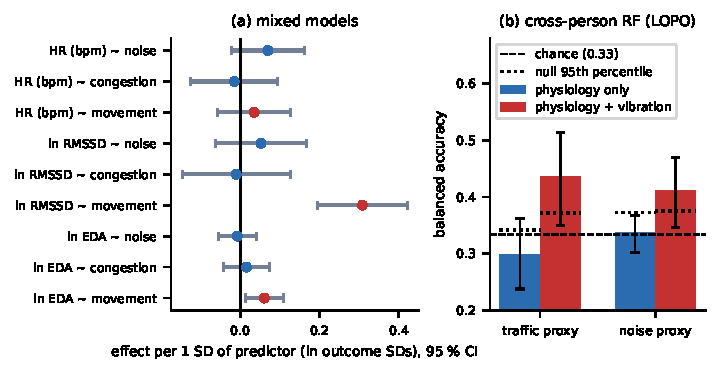
\includegraphics[width=0.92\textwidth]{figs/fig5_models.pdf}
\caption{(a) Effects from mixed models with a random intercept per session ($n=318$ non-overlapping windows from 11 sessions for HR and ln RMSSD; 200 for EDA), per SD of the predictor and expressed in SDs of the outcome, with 95\,\% CIs. Noise and congestion effects are not distinguishable from zero; movement (red) affects ln RMSSD and EDA. (b) Cross-person BA with 95\,\% CIs; dashed line: chance; dotted ticks: 95th percentile of the block-permutation null. Only models that see vibration exceed it.}
\label{fig:models}
\end{figure}

Mixed models (Fig.~\ref{fig:models}a) quantify the effects directly. Per standard deviation of within-person noise level, HR changes by $+0.99$~bpm (95\,\% CI $-0.32$ to $+2.30$, $p=0.14$); congestion by $-0.22$~bpm ($-1.78$ to $+1.35$). With 11 sessions the minimum detectable effect (80\,\% power) is about 1.9~bpm for noise and 2.2~bpm for congestion, so smaller effects cannot be excluded. Session explains a large share of the variance (intraclass correlation 0.57 for HR, 0.40 for ln RMSSD, 0.997 for skin temperature, 0.98 for EDA), which is why session-level effects dominate naive analyses. Movement, in contrast, increases ln RMSSD by 0.16 per SD (95\,\% CI 0.10--0.22, $p<0.001$) and ln EDA ($p=0.013$): since vibration should not raise vagal HRV, this is a motion artefact. Hour of day is confounded with participant and device (skin temperature rises $+5~^\circ$C per SD of hour) and is not interpretable.

\subsection{H2: the wrist accelerometer detects whether the bus is stopped}
\label{sec:h2}
H2 was specified as: stopped ($\geq$50\,\% of the window stopped) vs.\ moving ($<$10\,\%) windows can be separated from accelerometer features alone (log band powers 0.3--16~Hz and per-axis variability, standardised per participant, no hand orientation), with success defined as LOPO AUC $\geq$ 0.75 and $p<0.05$. We analysed 943 windows (439 stopped, 504 moving). The criterion was met (Fig.~\ref{fig:h2}): LOPO AUC 0.83 (logistic regression; 95\,\% CI over sessions 0.77--0.89) and 0.85 (random forest); LOSO AUC 0.84 and 0.85. The block-permutation null has mean AUC 0.57 (95th percentile 0.65), $p=0.0005$ (Holm-adjusted 0.004). Per participant AUC ranges from 0.80 to 1.00; per wristband it is 0.81 (P1, P4), 0.83 (P2) and 0.91 (P3), so there is no sign of a device-specific effect. Using only windows whose bus label was used as recorded ($n=358$) gives AUC 0.88, so the relabelling of some sessions does not drive the result.

The detector is essentially a vibration meter. A feature-group ablation (Supplement S5) shows that the 3--6~Hz band alone reaches AUC 0.83 and the SD of the magnitude alone 0.84, and removing any single group changes the AUC by less than 0.02. At a 0.5 threshold the error rate is 23\,\% (26.9\,\% of stopped and 20.0\,\% of moving windows). Errors are not concentrated near the class boundary: windows stopped more than 90\,\% of the time have the highest error (33.7\,\%), consistent with a bus idling with passengers moving; error grows slightly with GPS uncertainty (21.2\,\% if accuracy is $\leq5$~m, 26.9\,\% if $>10$~m); and one legacy session (P2-1, median GPS error 15.7~m) has chance-level discrimination (AUC 0.46 leave-one-participant-out, 0.55 leave-one-session-out), so part of the error is label noise in the GPS speed. Two sessions (P2-1 and P1-3) are at chance level in both validation schemes (AUC 0.46--0.55). Speed regression is weak (Spearman 0.49) and is reported in the Supplement.

\begin{figure}[t]
\centering
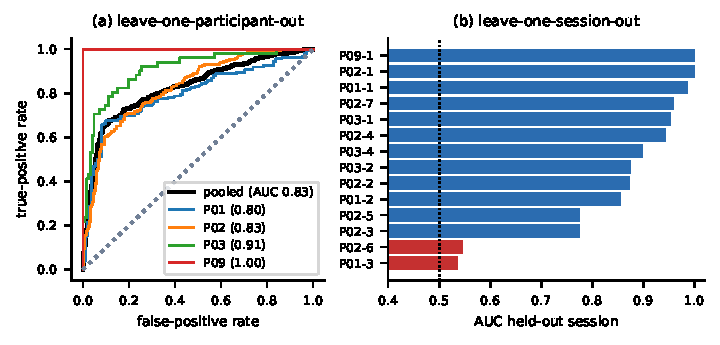
\includegraphics[width=0.92\textwidth]{figs/fig3_h2.pdf}
\caption{Vehicle-state detection from the wrist accelerometer (logistic regression). (a) ROC curves of held-out participants and pooled (AUC in legend; dotted: chance). (b) AUC for each held-out session (P$k$-$j$: $j$-th session of participant $k$; sessions are numbered chronologically, and the two legacy-format sessions of P2 (P2-1 and P2-2) are marked with an asterisk); red bars mark sessions near chance.}
\label{fig:h2}
\end{figure}

\subsection{H1: no cardiac response to noise bursts can be established}
H1 asked whether HR rises after noise bursts, using a within-session event design that avoids between-session confounding. Bursts were defined as seconds where the noise level exceeds its 60-s rolling median by $\geq$6~dB and lies in the top 10\,\% of the session (events $\geq$30~s apart, inside bus segments). HR was estimated at 1~Hz from 10-s spectral windows (quality index $\geq0.30$). The outcome is $\Delta$HR = mean HR in $[+3,+15]$~s minus mean HR in $[-10,-2]$~s, compared with all eligible control instants at least 30~s from any event; uncertainty comes from bootstrapping sessions and significance from circular shifts of the noise series (500). With the pre-specified thresholds only 81 events in 5 sessions were available, and the contrast was $+1.71$~bpm (95\,\% CI $-0.66$ to $+3.56$; $p=0.34$; $-0.24$~bpm after adjusting for movement change). Two looser variants, reported as sensitivity analyses, gave $-1.05$~bpm (188 events in 9 sessions; 95\,\% CI $-5.42$ to $+2.23$) and $-1.87$~bpm (250 events, 10 sessions; $-4.55$ to $+0.86$) (Fig.~\ref{fig:h1}; Supplement S7), and no dose--response relationship with burst intensity exists (Spearman 0.04). The minimum detectable effect is 3.0~bpm for the primary analysis; the Bayes factor in favour of no effect is 0.8--1.2 for priors with SD 1--4~bpm, i.e.\ the data are \emph{inconclusive}: they neither support a response nor rule out one of a few bpm. The result should be read as ``not established'', not as ``absent''.

\begin{figure}[t]
\centering
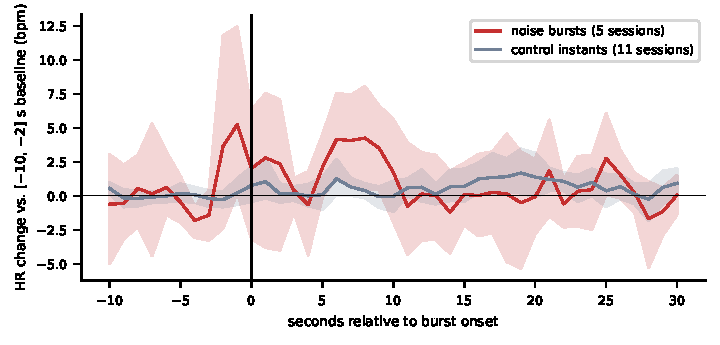
\includegraphics[width=0.68\textwidth]{figs/fig4_h1.pdf}
\caption{H1: mean HR change around noise bursts (red) and around control instants (grey) with 95\,\% bootstrap bands over sessions (5 sessions with at least 3 bursts; 11 for controls). HR is estimated in 10-s windows, so temporal resolution is about $\pm5$~s and the rise just before onset reflects this smoothing and estimation noise; the band for bursts includes zero at every lag.}
\label{fig:h1}
\end{figure}

\subsection{Pulse quality depends on the vehicle state (exploratory)}
Windows with valid HR are more frequent when the bus is stopped (88\,\%) than when it moves (80\,\%). The direction is the same for all participants (stopped vs.\ moving: P1 82/72\,\%, P2 94/89\,\%, P3 80/76\,\%, P4 100/48\,\%). The mean within-participant difference is $+17.8$ percentage points (95\,\% CI over sessions $+9.6$ to $+26.4$) but it is dominated by P4, who has few windows (13 and 25); excluding P4 it is $+6.4$ points (95\,\% CI $-5.1$ to $+17.9$), which is not distinguishable from zero. We therefore treat the effect on pulse validity as suggestive only.

\section{Threats to Validity}
\label{sec:threats}
\emph{Internal.} (i)~PPG and EDA decoding is validated by physical criteria but not against ECG or a reference EDA device; this is a major limitation and absolute HR/HRV values must not be interpreted clinically. (ii)~Session, person and wristband are confounded (three wristbands for four people; hour of day is tied to participant); we mitigate this with within-person normalisation, session random effects and held-out validation. (iii)~Vibration affects HRV and EDA. (iv)~Overlapping windows are handled by block permutation and non-overlapping subsets, but the effective sample size is smaller than the number of rows.
\emph{Construct.} The proxies come from phone sensors and are not stress labels; the microphone level is uncalibrated; GPS speed is noisy; and the traffic proxy is physically coupled to vibration, so the gain from vibration features is partly expected and is not a physiological finding.
\emph{Selection.} The bus-only criterion, the relabelling of five sessions and the exclusion of two sessions were fixed for data-quality reasons but could favour well-recorded trips; H2 holds on windows whose label was used as recorded (AUC 0.88).
\emph{External.} Four volunteers from the research environment, 15 sessions, one city and one device model limit generalisation.
\emph{Statistical.} With 11 sessions the minimum detectable effects (about 2~bpm for noise and congestion, 3~bpm for burst responses) are not small, so null results mean ``not established''. Multiplicity is controlled with Holm within two declared families; descriptive analyses are uncorrected.

\section{Discussion}
What the wrist reliably senses on a bus is the \emph{vehicle}. Vehicle state can be recovered from the accelerometer across persons and sessions, whereas physiological features alone carry no detectable information about traffic or noise proxies when the person or session is new. Several innocuous-looking practices would have produced a misleading headline here: global normalisation, evaluating clusters on the sessions they were formed on, including the first minutes of EDA, permuting overlapping windows one by one, and feeding movement features to a model later interpreted as physiological. Table~\ref{tab:recs} turns these observations into recommendations. The detector could also gate windows whose physiological features are less reliable, although the evidence that pulse validity drops while the bus moves is only suggestive.

\begin{table}[t]
\caption{Recommendations for wearable stress studies in transit, with the evidence from this study.}
\label{tab:recs}
\centering
\footnotesize
\setlength{\tabcolsep}{3pt}
\begin{tabular}{>{\raggedright\arraybackslash}p{2.3cm}>{\raggedright\arraybackslash}p{4.9cm}>{\raggedright\arraybackslash}p{4.4cm}}
\toprule
Issue & Evidence here & Recommendation\\
\midrule
Person and device baselines & Global normalisation gives person-driven clusters & Standardise within person; log device\\
Session effects & Clusters align with sessions (NMI 0.36--0.43 vs.\ 0.12--0.14 with traffic); ICC 0.98--0.997 for EDA and temperature & Validate on held-out sessions; add session random effects\\
Sensor warm-up & EDA falls from about 7 to 2~$\mu$S in minutes & Discard the first 5 min of EDA\\
Vibration artefacts & Movement raises ln RMSSD by 0.16 SD per SD & Use the accelerometer to flag windows; do not interpret HRV in motion\\
Context leakage & Physiology-only BA 0.21--0.38 (chance) vs.\ 0.41--0.44 with vibration & Report models with and without accelerometer features\\
Overlapping windows & Block-permutation null AUC mean 0.57, not 0.50 & Use block permutations and non-overlapping subsets\\
Raw logging & Layouts inferred; one format unresolved & Log raw packets; validate against ECG\\
\bottomrule
\end{tabular}
\end{table}

\emph{Future work.} (i)~Record a simultaneous chest-strap ECG in at least ten rides to validate PPG-derived HR and HRV; (ii)~calibrate the phone microphone against a sound-level meter; (iii)~use the smartphone IMU as a second vibration channel to separate vehicle from wrist motion; (iv)~recruit at least 30 participants on several routes, in more than one city and on other vehicle types (e.g., metro and rail), one wristband per person, to test whether the vehicle-state detector and the negative physiological findings generalise; (v)~collect momentary self-reports as stress labels; (vi)~obtain the manufacturer's specification of the second EDA format.

\section{Conclusions}
We built and validated a pipeline from raw wristband packets to context-aware windows in real bus rides. The wrist accelerometer detects vehicle state (AUC 0.83--0.85), whereas physiology alone neither predicts traffic, noise or exposure proxies in unseen persons nor shows an established response to noise bursts, and motion contaminates HRV. These findings, together with the threats to validity listed above, argue for within-person normalisation, session-held-out validation and explicit control of motion in transit studies.

\paragraph{Ethics, privacy and availability.} Participants were adult volunteers who gave informed consent; only pseudonymous identifiers are stored; microphone audio was never recorded (only a level), and GPS is retained only as per-window means. Code, analysis protocols and the Supplement (S1--S9) are available at \url{https://github.com/MelanyCN/wearable-stress-public-transport}; the code reproduces all tables and figures from the raw logs. The data are available from the authors upon reasonable request.

\begin{thebibliography}{16}
\bibitem{schmidt2018} Schmidt, P., Reiss, A., Duerichen, R., Marberger, C., Van Laerhoven, K.: Introducing WESAD, a multimodal dataset for wearable stress and affect detection. In: Proc. 20th ACM Int. Conf. on Multimodal Interaction, pp.~400--408 (2018). \doi{10.1145/3242969.3242985}
\bibitem{iqbal2022} Iqbal, T., Elahi, A., Wijns, W., Shahzad, A.: Exploring unsupervised machine learning classification methods for physiological stress detection. Front. Med. Technol. 4, 782756 (2022). \doi{10.3389/fmedt.2022.782756}
\bibitem{bosch2025} Bosch, E., Luther, A.R., Ihme, K.: Travel experience in public transport: experience sampling and cardiac activity data for spatial analysis. Sci. Data 12, 633 (2025). \doi{10.1038/s41597-025-04955-4}
\bibitem{wang2023} Wang, A.L., Bista, S., Can, A., Chaix, B.: Personal noise exposure during daily commutes and subjectively reported stress: a trip stage level analysis of MobiliSense data. J. Transp. Health 30, 101612 (2023). \doi{10.1016/j.jth.2023.101612}
\bibitem{vos2023} Vos, G., Trinh, K., Sarnyai, Z., Rahimi Azghadi, M.: Generalizable machine learning for stress monitoring from wearable devices: a systematic literature review. Int. J. Med. Inform. 173, 105026 (2023). \doi{10.1016/j.ijmedinf.2023.105026}
\bibitem{amin2025} Amin, O.B., Mishra, V., Tapera, T.M., Volpe, R., Sathyanarayana, A.: Extending stress detection reproducibility to consumer wearable sensors. In: IEEE EMBC 2025. arXiv:2505.05694 (2025)
\bibitem{schuurmans2020} Schuurmans, A.A.T., de Looff, P., Nijhof, K.S., et al.: Validity of the Empatica E4 wristband to measure heart rate variability (HRV) parameters: a comparison to electrocardiography (ECG). J. Med. Syst. 44, 190 (2020)
\bibitem{costantini2023} Costantini, S., Chiappini, M., Malerba, G., Dei, C., Falivene, A., Arlati, S., Colombo, V., Biffi, E., Storm, F.A.: Wrist-worn sensor validation for heart rate variability and electrodermal activity detection in a stressful driving environment. Sensors 23(20), 8423 (2023). \doi{10.3390/s23208423}
\bibitem{bosch2026} Bosch, E.: Separating acute psychological stress from physical exertion in biometric signals. arXiv:2605.15756 (2026), preprint
\bibitem{gholami2020} Gholamiangonabadi, D., Kiselov, N., Grolinger, K.: Deep neural networks for human activity recognition with wearable sensors: leave-one-subject-out cross-validation for model selection. IEEE Access 8, 133982--133994 (2020)
\bibitem{ojala2010} Ojala, M., Garriga, G.C.: Permutation tests for studying classifier performance. J. Mach. Learn. Res. 11, 1833--1863 (2010)
\bibitem{holm1979} Holm, S.: A simple sequentially rejective multiple test procedure. Scand. J. Stat. 6(2), 65--70 (1979)
\bibitem{virtanen2020} Virtanen, P., et al.: SciPy 1.0: fundamental algorithms for scientific computing in Python. Nat. Methods 17, 261--272 (2020)
\bibitem{sklearn2011} Pedregosa, F., et al.: Scikit-learn: machine learning in Python. J. Mach. Learn. Res. 12, 2825--2830 (2011)
\bibitem{seabold2010} Seabold, S., Perktold, J.: statsmodels: econometric and statistical modeling with Python. In: Proc. 9th Python in Science Conf., pp.~92--96 (2010)
\end{thebibliography}
\end{document}
